\documentclass[12pt,a4paper]{article}

%% ── Pacotes ────────────────────────────────────────────────────────────────
\usepackage[utf8]{inputenc}
\usepackage[T1]{fontenc}
\usepackage[brazil]{babel}
\usepackage{lmodern}
\usepackage{geometry}
\usepackage{graphicx}
\usepackage{amsmath,amssymb}
\usepackage{booktabs}
\usepackage{tabularx}
\usepackage{multirow}
\usepackage{array}
\usepackage[dvipsnames]{xcolor}
\usepackage[most]{tcolorbox}
\usepackage{listings}
\usepackage{hyperref}
\usepackage{float}
\usepackage{caption}
\usepackage{subcaption}
\usepackage{enumitem}
\usepackage{fancyhdr}
\usepackage{titlesec}

\geometry{top=2.5cm, bottom=2.5cm, left=3cm, right=2.5cm}

%% ── Cores ──────────────────────────────────────────────────────────────────
\definecolor{azul}    {RGB}{50,100,180}
\definecolor{vermelho}{RGB}{200,60,40}
\definecolor{verde}   {RGB}{40,140,60}
\definecolor{laranja} {RGB}{200,120,0}
\definecolor{roxo}    {RGB}{120,40,160}
\definecolor{cinza}   {RGB}{100,100,100}
\definecolor{fundo}   {RGB}{248,249,252}
\definecolor{fundoazul}{RGB}{235,244,255}
\definecolor{fundoverde}{RGB}{235,248,238}
\definecolor{fundovermelho}{RGB}{255,240,238}
\definecolor{fundolaranja}{RGB}{255,248,230}

%% ── Caixas coloridas ───────────────────────────────────────────────────────
\tcbset{
  notabox/.style={
    colback=fundoazul, colframe=azul, coltitle=white,
    fonttitle=\bfseries\small, title={Nota Técnica},
    boxrule=1pt, arc=3pt, left=6pt, right=6pt, top=4pt, bottom=4pt},
  codigobox/.style={
    colback=gray!8, colframe=cinza!60, coltitle=white,
    fonttitle=\bfseries\small,
    boxrule=0.8pt, arc=3pt, left=6pt, right=6pt, top=4pt, bottom=4pt},
  equacaobox/.style={
    colback=fundoverde, colframe=verde, coltitle=white,
    fonttitle=\bfseries\small,
    boxrule=1pt, arc=3pt, left=6pt, right=6pt, top=4pt, bottom=4pt},
  atencaobox/.style={
    colback=fundovermelho, colframe=vermelho, coltitle=white,
    fonttitle=\bfseries\small, title={Atenção ASIL-B},
    boxrule=1pt, arc=3pt, left=6pt, right=6pt, top=4pt, bottom=4pt},
  dbc/.style={
    colback=gray!5, colframe=azul!40,
    boxrule=0.6pt, arc=2pt, left=4pt, right=4pt, top=3pt, bottom=3pt,
    fontupper=\ttfamily\small},
}

%% ── Código-fonte ───────────────────────────────────────────────────────────
\lstdefinestyle{matlab}{
  language=Matlab, basicstyle=\ttfamily\footnotesize,
  keywordstyle=\color{azul}\bfseries,
  commentstyle=\color{OliveGreen!80!black}\itshape,
  stringstyle=\color{vermelho},
  numbers=left, numberstyle=\tiny\color{gray},
  breaklines=true, frame=single, rulecolor=\color{gray!40},
  backgroundcolor=\color{gray!5}, xleftmargin=1.5em,
}
\lstdefinestyle{dbc}{
  basicstyle=\ttfamily\small,
  numbers=none, frame=single, rulecolor=\color{azul!30},
  backgroundcolor=\color{fundoazul},
  breaklines=true,
}
\lstset{style=matlab}

%% ── Cabeçalho ──────────────────────────────────────────────────────────────
\pagestyle{fancy}
\fancyhf{}
\fancyhead[L]{\small\color{cinza}Sistema AEB --- Barramento CAN}
\fancyhead[R]{\small\color{cinza}Residência Stellantis/UFPE 2026}
\fancyfoot[C]{\small\thepage}
\renewcommand{\headrulewidth}{0.4pt}

%% ── Títulos ────────────────────────────────────────────────────────────────
\titleformat{\section}{\large\bfseries\color{azul}}{{\thesection}}{0.8em}{}
\titleformat{\subsection}{\normalsize\bfseries\color{azul!70!black}}{{\thesubsection}}{0.7em}{}

%% ── Hyperlinks ─────────────────────────────────────────────────────────────
\hypersetup{colorlinks=true, linkcolor=azul, urlcolor=azul, citecolor=verde}

%% ═══════════════════════════════════════════════════════════════════════════
\begin{document}

%% ── Capa ───────────────────────────────────────────────────────────────────
\begin{titlepage}
  \centering
  \vspace*{1cm}
  {\color{azul}\rule{\linewidth}{2pt}}\\[0.5cm]
  {\Huge\bfseries\color{azul} Barramento CAN do Sistema AEB}\\[0.3cm]
  {\Large\color{cinza} Modelagem e Simulação em Simulink}\\[0.2cm]
  {\color{azul}\rule{\linewidth}{1pt}}\\[1cm]

  {\large
  \begin{tabular}{ll}
    \textbf{Projeto:}  & Residência Tecnológica Stellantis/UFPE\\[4pt]
    \textbf{Módulo:}   & Modelagem --- Barramento CAN\\[4pt]
    \textbf{Data:}     & Março de 2026\\[4pt]
    \textbf{Norma:}    & ISO~11898 (CAN), AUTOSAR, ISO~26262 ASIL-B\\[4pt]
    \textbf{Arquivo:}  & \texttt{AEB\_CAN.slx}\\[4pt]
    \textbf{DBC:}      & \texttt{can/aeb\_system.dbc} --- 500~kbps\\
  \end{tabular}
  }\\[1.5cm]

  \begin{tcolorbox}[notabox, width=0.85\linewidth]
    Este documento descreve o modelo Simulink do barramento CAN do sistema AEB,
    com foco na codificação/decodificação de sinais conforme o arquivo DBC,
    no mecanismo de AliveCounter, no CRC-4 da mensagem ASIL-B e na
    injeção e detecção de falhas de comunicação.
  \end{tcolorbox}

  \vfill
  {\color{cinza}\small Gerado com MATLAB R2025b + Simulink}
\end{titlepage}

\tableofcontents
\newpage

%% ═══════════════════════════════════════════════════════════════════════════
\section{Introdução}
\label{sec:intro}

O barramento CAN (\textit{Controller Area Network}) é a espinha dorsal de
comunicação do sistema AEB. No veículo real, nenhum módulo acessa diretamente
os dados de outro: toda informação transita pelo barramento com temporização
cíclica, fator de escala e mecanismos de integridade. A modelagem Simulink
deste subsistema tem dois objetivos principais:

\begin{enumerate}
  \item \textbf{Verificação de codificação}: confirmar que os fatores, offsets
    e tamanhos de bit definidos no arquivo DBC são aplicados corretamente em
    ambos os sentidos (TX e RX).
  \item \textbf{Injeção e detecção de falhas}: validar que os mecanismos de
    AliveCounter e CRC-4 detectam corrupção de mensagem e perda de frame,
    gerando os DTCs correspondentes conforme ISO~14229 (UDS).
\end{enumerate}

\begin{figure}[H]
  \centering
  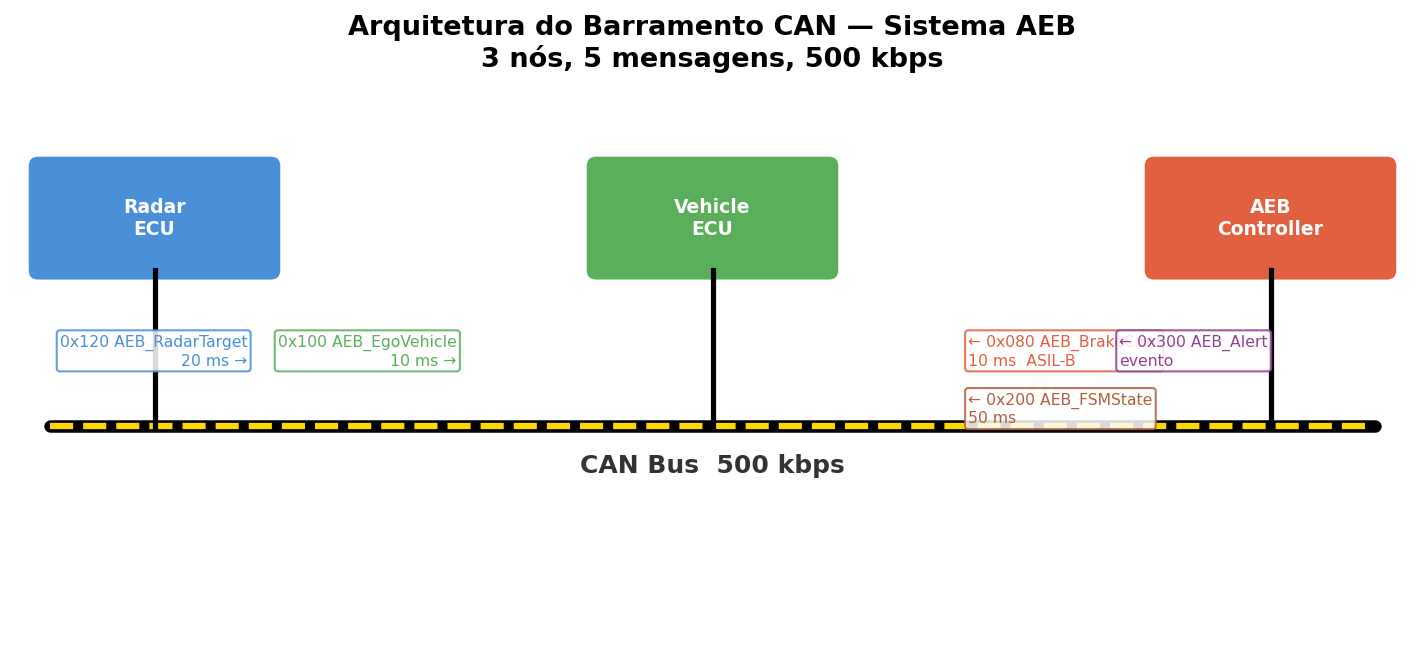
\includegraphics[width=\linewidth]{fig_arquitetura_can.png}
  \caption{Arquitetura do barramento CAN do sistema AEB: 3 nós, 5 mensagens,
           500~kbps.}
  \label{fig:arquitetura}
\end{figure}

\begin{tcolorbox}[notabox]
  O arquivo de banco de dados CAN \texttt{aeb\_system.dbc} é a fonte de
  verdade formal para todos os parâmetros de sinalização. Qualquer
  discrepância entre o modelo Simulink e o DBC deve ser resolvida em favor
  do DBC.
\end{tcolorbox}

%% ═══════════════════════════════════════════════════════════════════════════
\section{Barramento CAN --- Visão Geral}
\label{sec:visao}

\subsection{Configuração do barramento}

\begin{center}
\begin{tabular}{ll}
  \toprule
  \textbf{Parâmetro}   & \textbf{Valor} \\
  \midrule
  Velocidade           & 500~kbps \\
  Nós                  & \texttt{AEB\_Controller}, \texttt{Vehicle\_ECU}, \texttt{Radar\_ECU} \\
  Mensagens            & 5 (cíclicas + evento) \\
  Comprimento máximo   & 8 bytes (CAN clássico) \\
  Norma                & ISO~11898-1 \\
  \bottomrule
\end{tabular}
\end{center}

\subsection{Temporização das mensagens}

\begin{figure}[H]
  \centering
  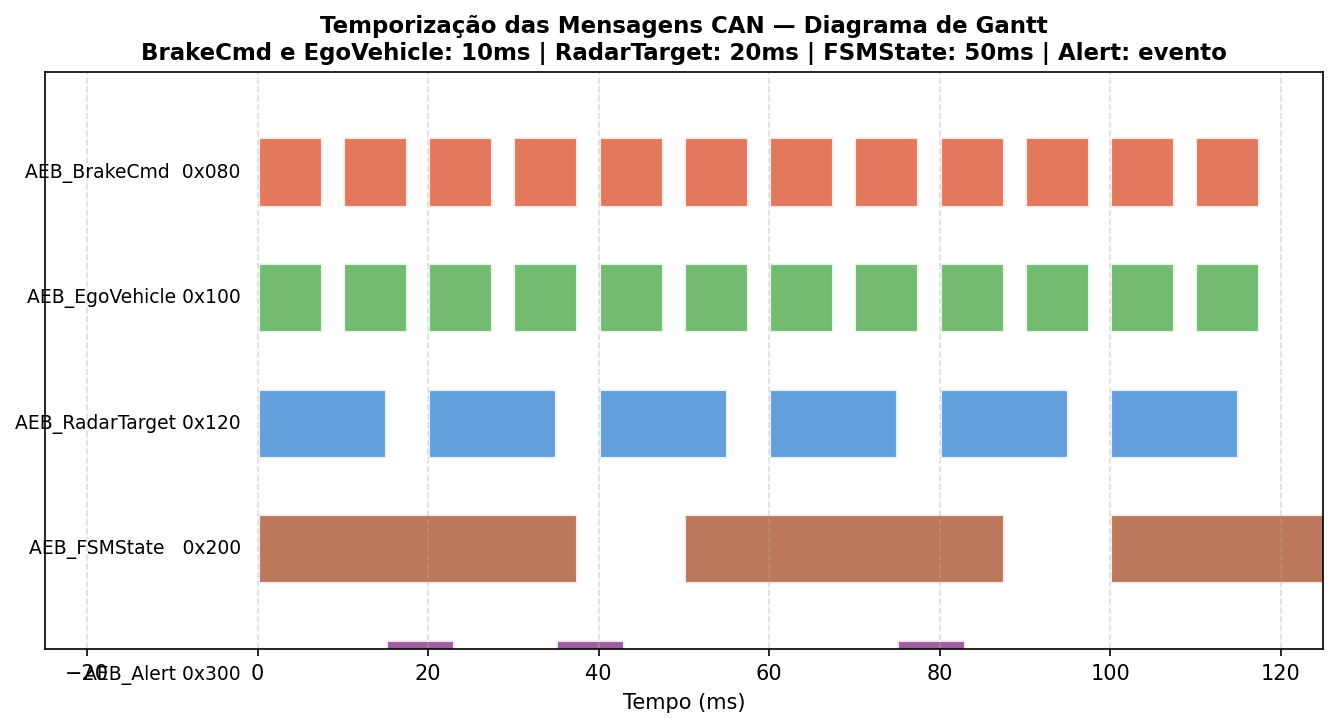
\includegraphics[width=\linewidth]{fig_timing_can.png}
  \caption{Diagrama de Gantt --- temporização das 5 mensagens CAN.
           \texttt{AEB\_BrakeCmd} e \texttt{AEB\_EgoVehicle} a 10~ms;
           \texttt{AEB\_RadarTarget} a 20~ms; \texttt{AEB\_FSMState} a 50~ms;
           \texttt{AEB\_Alert} dirigida por evento.}
  \label{fig:timing}
\end{figure}

A Figura~\ref{fig:timing} evidencia uma consequência importante da
assincronismo entre \texttt{AEB\_EgoVehicle} (10~ms) e
\texttt{AEB\_RadarTarget} (20~ms): o controlador AEB deve manter
\texttt{v\_target\_cached\_}, calculado dentro do \textit{callback} do radar,
para garantir que velocidade do ego e velocidade relativa sejam
contemporâneas no cálculo de TTC.

%% ═══════════════════════════════════════════════════════════════════════════
\section{Detalhamento das Mensagens}
\label{sec:mensagens}

\subsection{AEB\_BrakeCmd --- 0x080 (ASIL-B)}

Mensagem de segurança crítica: carrega o comando de frenagem do
\texttt{AEB\_Controller} para o atuador de freio. Protegida por
AliveCounter e CRC de 4~bits.

\begin{tcolorbox}[dbc]
BO\_ 128 AEB\_BrakeCmd: 4 AEB\_Controller\\
\ SG\_ BrakeRequest  : 0|1@1+  (1,0)   [0|1]      ""   Vehicle\_ECU\\
\ SG\_ BrakePressure : 1|15@1+ (0.1,0) [0|3276.7] "bar" Vehicle\_ECU\\
\ SG\_ BrakeMode     : 16|3@1+ (1,0)   [0|7]      ""   Vehicle\_ECU\\
\ SG\_ AliveCounter  : 24|4@1+ (1,0)   [0|15]     ""   Vehicle\_ECU\\
\ SG\_ CRC           : 28|4@1+ (1,0)   [0|15]     ""   Vehicle\_ECU
\end{tcolorbox}

\begin{tcolorbox}[atencaobox]
  A mensagem \texttt{AEB\_BrakeCmd} é classificada como ASIL-B.
  O receptor (\texttt{Vehicle\_ECU}) deve rejeitar o frame imediatamente
  ao detectar CRC incorreto ou AliveCounter com diferença $\neq 1 \pmod{16}$.
  Falha no AliveCounter por $>$5~ciclos activa o DTC C1005; erro de CRC
  activa C1004.
\end{tcolorbox}

\subsection{AEB\_EgoVehicle --- 0x100}

\begin{tcolorbox}[dbc]
BO\_ 256 AEB\_EgoVehicle: 8 Vehicle\_ECU\\
\ SG\_ VehicleSpeed   : 0|16@1+  (0.01,0)       [0|655.35]     "m/s"\\
\ SG\_ LongAccel      : 16|16@1+ (0.001,-32)    [-32|33.535]   "m/s\textasciicircum{}2"\\
\ SG\_ YawRate        : 32|16@1+ (0.01,-327.68) [-327.68|327.67] "deg/s"\\
\ SG\_ SteeringAngle  : 48|16@1+ (0.1,-3276.8)  [-3276.8|3276.7] "deg"
\end{tcolorbox}

A aceleração longitudinal usa \textit{offset} de $-32$~m/s$^2$ para
representar valores negativos em campo sem sinal:
$\text{raw} = \lfloor(\text{físico} + 32) / 0{,}001\rceil$.

\subsection{AEB\_RadarTarget --- 0x120}

\begin{tcolorbox}[dbc]
BO\_ 288 AEB\_RadarTarget: 8 Radar\_ECU\\
\ SG\_ TargetDistance : 0|16@1+  (0.01,0)      [0|655.35]     "m"\\
\ SG\_ RelativeSpeed  : 16|16@1+ (0.01,-327.68) [-327.68|327.67] "m/s"\\
\ SG\_ TTC            : 32|16@1+ (0.001,0)     [0|65.535]     "s"\\
\ SG\_ Confidence     : 48|8@1+  (1,0)         [0|15]         ""
\end{tcolorbox}

\subsection{AEB\_FSMState --- 0x200}

\begin{center}
\begin{tabular}{cll}
  \toprule
  \textbf{FSMState} & \textbf{Nome} & \textbf{Descrição} \\
  \midrule
  0 & OFF       & Sistema desligado \\
  1 & STANDBY   & Aguardando ameaça \\
  2 & WARNING   & Alerta ao motorista \\
  3 & BRAKE\_L1 & Frenagem leve: $-2$~m/s$^2$ \\
  4 & BRAKE\_L2 & Frenagem moderada: $-4$~m/s$^2$ \\
  5 & BRAKE\_L3 & Frenagem total: $-6$~m/s$^2$ \\
  6 & POST\_BRAKE& Manutenção pós-parada \\
  \bottomrule
\end{tabular}
\end{center}

\subsection{AEB\_Alert --- 0x300 (evento)}

Publicada apenas em mudanças de estado FSM. Comanda o HMI de alertas
visuais (\textit{BuzzerCmd}): SingleBeep (WARNING), DoubleBeep (L1),
FastPulse (L2), ContinuousBeep (L3).

%% ═══════════════════════════════════════════════════════════════════════════
\section{Codificação DBC}
\label{sec:codificacao}

\subsection{Princípio de codificação}

O padrão DBC define para cada sinal: posição inicial em bits, comprimento
em bits, endianness (\texttt{@1} = little-endian), sinalidade
(\texttt{+} = sem sinal), fator e \textit{offset}:

\begin{tcolorbox}[equacaobox, title={Fórmula DBC}]
\begin{equation}
  \text{valor\_físico} = \text{raw} \times \text{fator} + \text{offset}
\end{equation}
\begin{equation}
  \text{raw} = \left\lfloor \frac{\text{valor\_físico} - \text{offset}}
                                  {\text{fator}} \right\rceil
\end{equation}
Exemplo: $\texttt{VehicleSpeed} = 10{,}0\;\text{m/s}
  \;\Rightarrow\; \text{raw} = \lfloor 10{,}0 / 0{,}01 \rceil = 1000$.
\end{tcolorbox}

\begin{figure}[H]
  \centering
  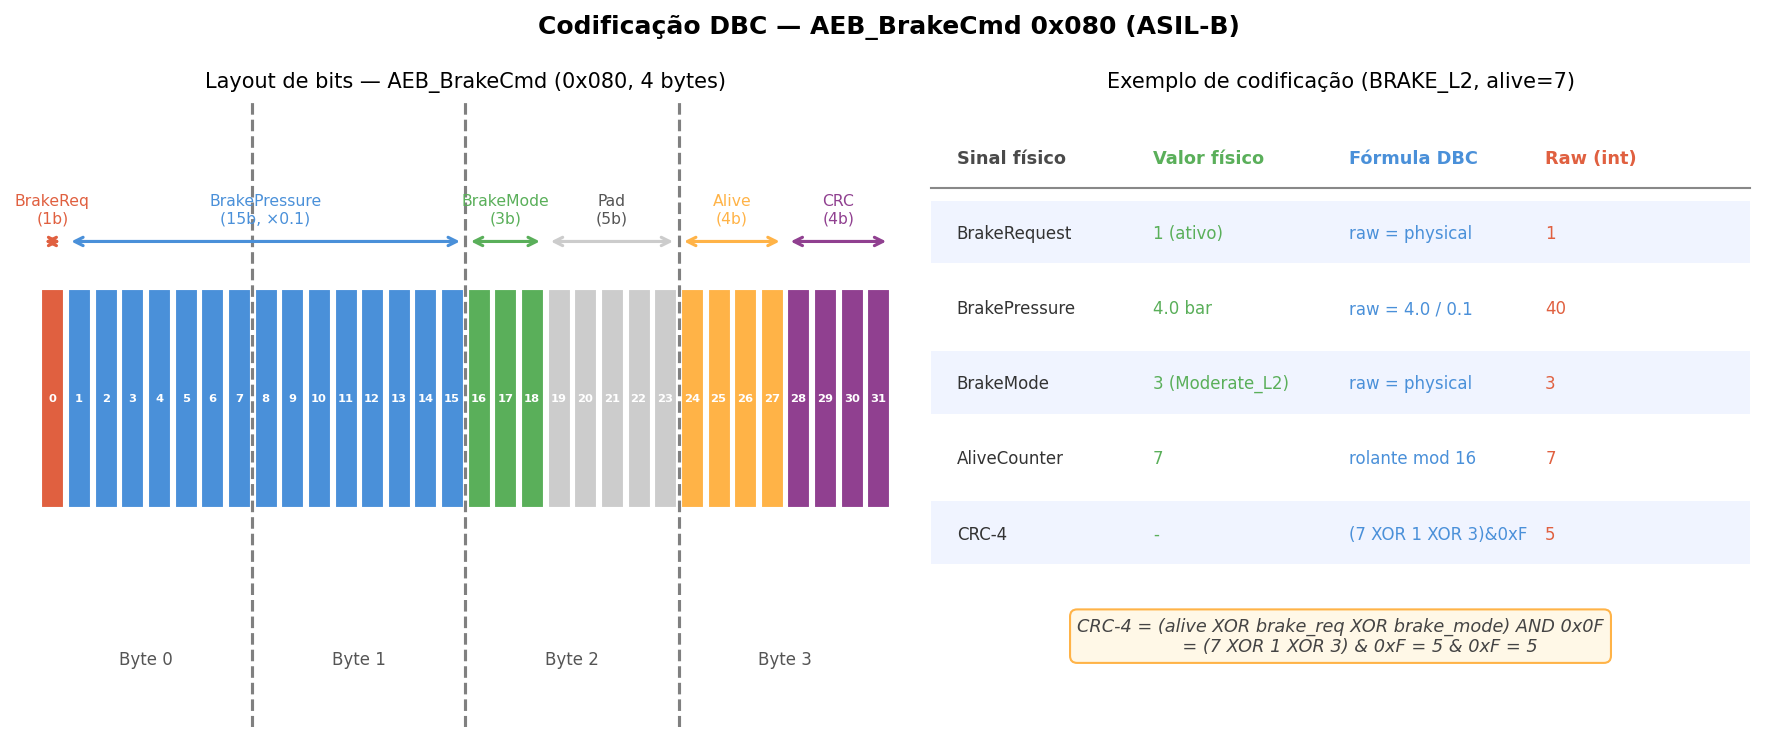
\includegraphics[width=\linewidth]{fig_codificacao_dbc.png}
  \caption{Layout de bits do frame \texttt{AEB\_BrakeCmd} (4~bytes) e
           exemplo numérico de codificação para BRAKE\_L2.}
  \label{fig:codificacao}
\end{figure}

\subsection{Implementação no Simulink}

No bloco \texttt{TX\_BrakeCmd}, o bloco MATLAB Function implementa:

\begin{lstlisting}[style=matlab, caption={Codificação DBC em MATLAB Function}]
% BrakeRequest: 1 bit, sem fator/offset
bc_req_r   = double(brake_req > 0);

% BrakePressure: 15 bits, fator 0.1, range 0-3276.7 bar
bc_press_r = double(min(round(brake_press / 0.1), 32767));

% BrakeMode: 3 bits (0=Off, 1=Warning, 2=L1, 3=L2, 4=L3)
bc_mode_r  = double(min(max(round(brake_mode), 0), 5));
\end{lstlisting}

%% ═══════════════════════════════════════════════════════════════════════════
\section{AliveCounter}
\label{sec:alive}

\subsection{Mecanismo}

O AliveCounter é um campo de 4~bits presente em \texttt{AEB\_BrakeCmd}
e \texttt{AEB\_RadarTarget}. Incrementa a cada frame transmitido,
reiniciando de 15 para 0 (contador rolante módulo~16):

\begin{tcolorbox}[equacaobox, title={AliveCounter}]
\begin{equation}
  \text{alive}_{k+1} = (\text{alive}_k + 1) \bmod 16
\end{equation}
\textbf{Sequência esperada:} $0, 1, 2, \ldots, 14, 15, 0, 1, 2, \ldots$
\end{tcolorbox}

O receptor detecta falha quando dois valores consecutivos não diferem
por exatamente~1 módulo~16. Isso captura tanto \textbf{perda de frame}
(diferença $\geq 2$) quanto \textbf{travamento do transmissor}
(diferença $= 0$).

\begin{lstlisting}[style=matlab, caption={AliveCounter no TX (MATLAB Function)}]
persistent alive_cnt;
if isempty(alive_cnt), alive_cnt = uint8(0); end
alive = double(alive_cnt);
alive_cnt = bitand(alive_cnt + uint8(1), uint8(15));  % mod 16
\end{lstlisting}

\begin{lstlisting}[style=matlab, caption={Verificacao do AliveCounter no RX}]
persistent last_alive;
if isempty(last_alive), last_alive = -1; end
if last_alive < 0
    alive_err = 0;  % primeiro frame: sem referencia
else
    alive_err = double(alive ~= mod(last_alive + 1, 16));
end
last_alive = alive;
\end{lstlisting}

\subsection{Simulação}

\begin{figure}[H]
  \centering
  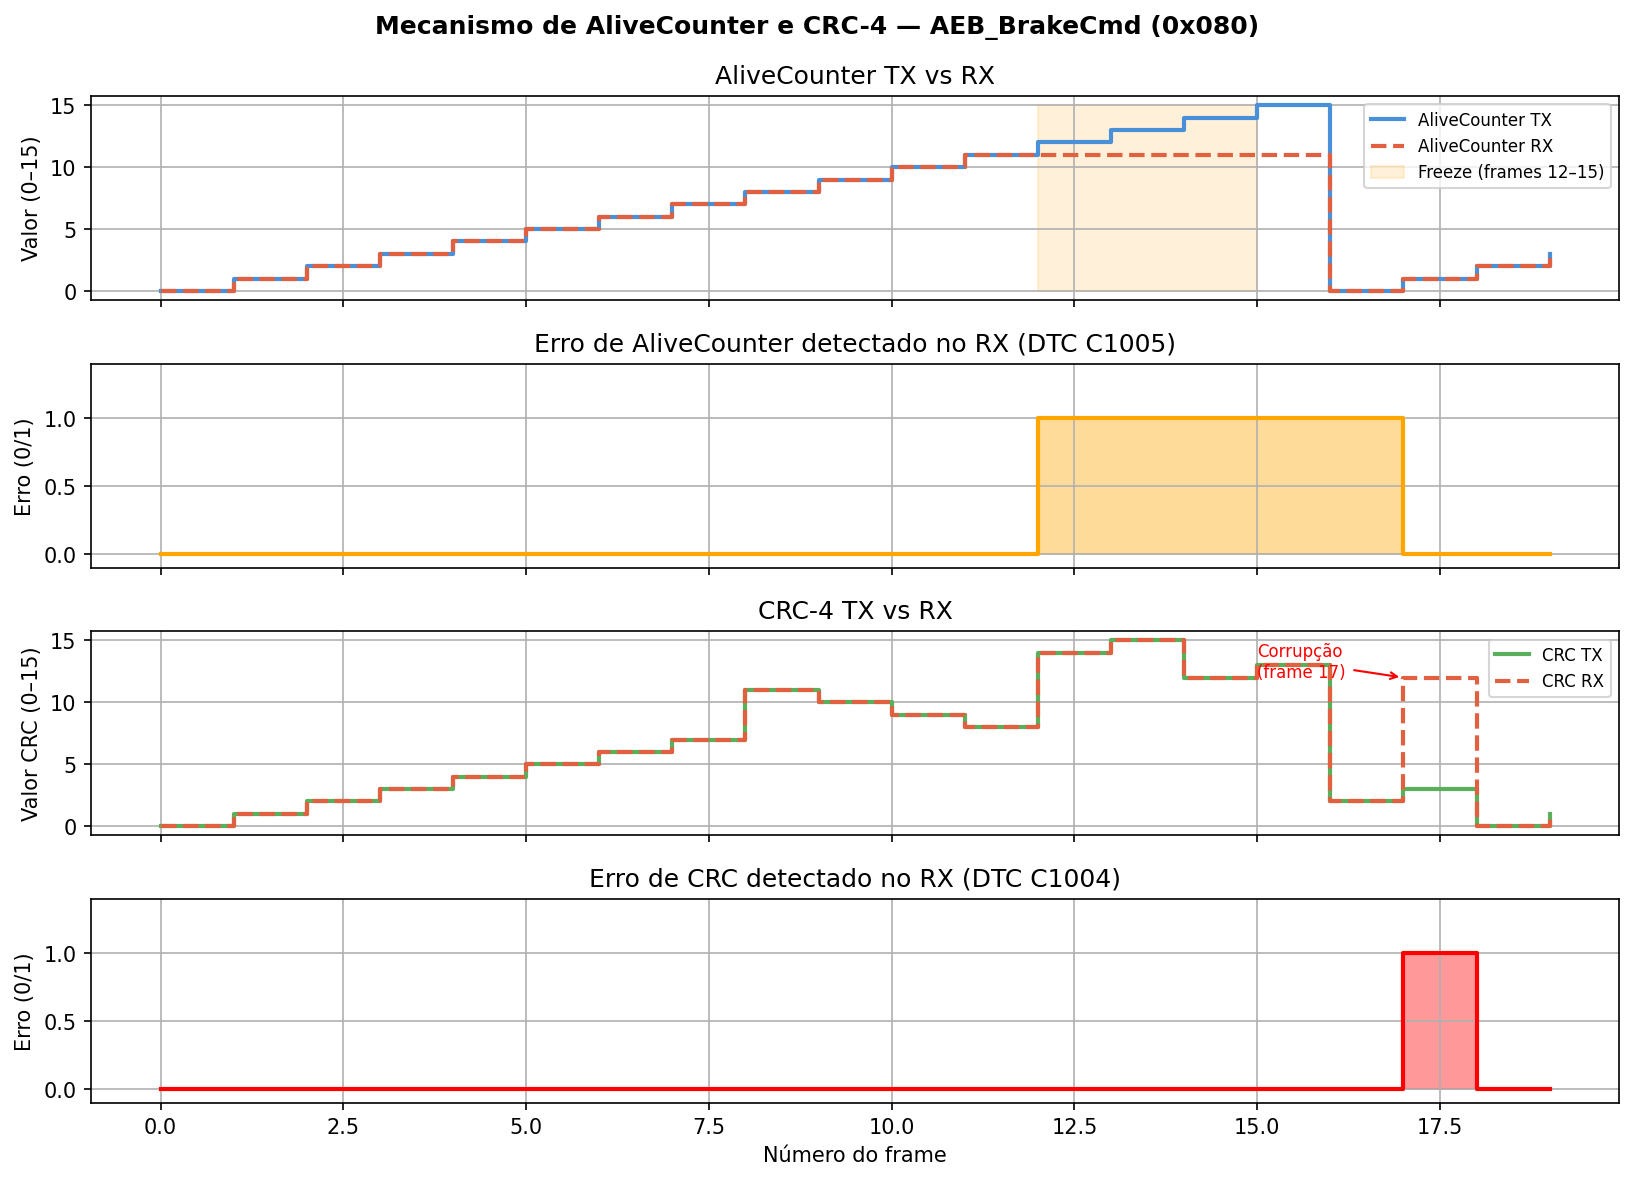
\includegraphics[width=\linewidth]{fig_alive_crc.png}
  \caption{Simulação do AliveCounter e CRC-4: freeze entre frames 12--15
           gera \texttt{alive\_err=1} (DTC~C1005); corrupção no frame~17
           gera \texttt{crc\_err=1} (DTC~C1004).}
  \label{fig:alive_crc}
\end{figure}

%% ═══════════════════════════════════════════════════════════════════════════
\section{CRC de 4 Bits}
\label{sec:crc}

O campo \texttt{CRC} de 4~bits na mensagem \texttt{AEB\_BrakeCmd} protege
a integridade dos três primeiros bytes de payload. É calculado por XOR
simples:

\begin{tcolorbox}[equacaobox, title={CRC-4 --- AEB\_BrakeCmd}]
\begin{equation}
  \text{CRC} = (\text{alive} \oplus \text{brake\_req} \oplus \text{brake\_mode})
               \;\&\; \texttt{0x0F}
\end{equation}
onde $\oplus$ denota XOR bit-a-bit e $\&\;\texttt{0x0F}$ extrai apenas
os 4 bits menos significativos.
\end{tcolorbox}

Esta função está definida em \texttt{aeb\_controller\_node.cpp}:
\begin{lstlisting}[style=matlab, caption={CRC-4 no bloco TX (MATLAB Function)}]
% b0=alive_counter, b1=brake_request, b2=brake_mode
crc = double(bitand( ...
    bitxor(bitxor(uint8(alive), uint8(bc_req_r)), uint8(bc_mode_r)), ...
    uint8(15)));  % mascara 0x0F
\end{lstlisting}

\begin{tcolorbox}[notabox]
  Embora o XOR de 4~bits não seja um CRC polinomial automotivo (como o
  CRC-8 SAE~J1939), é suficiente para detectar erros de bit único e
  serve como mecanismo educacional representativo de proteção de mensagem
  ASIL-B.
\end{tcolorbox}

%% ═══════════════════════════════════════════════════════════════════════════
\section{Injeção de Falhas}
\label{sec:falhas}

O subsistema \texttt{Injecao\_Falhas} implementa três tipos de falha
controláveis via sinais de workspace:

\begin{center}
\begin{tabularx}{\linewidth}{lXl}
  \toprule
  \textbf{Tipo} & \textbf{Descrição} & \textbf{DTC gerado} \\
  \midrule
  \texttt{fault\_dropout} & Supressão completa do frame
    (\texttt{valid=0}) & C1010 \\
  \texttt{fault\_crc} & Inversão de todos os 4~bits do CRC
    (XOR 0x0F) & C1004 \\
  \texttt{fault\_alive} & Congelamento do AliveCounter
    (valor não incrementa) & C1005 \\
  \bottomrule
\end{tabularx}
\end{center}

\begin{lstlisting}[style=matlab, caption={Falha de CRC no subsistema Injecao\_Falhas}]
if f_crc > 0
    crc_rx = double(bitxor(uint8(crc), uint8(15)));  % inverte 4 bits
else
    crc_rx = crc;
end
\end{lstlisting}

\begin{figure}[H]
  \centering
  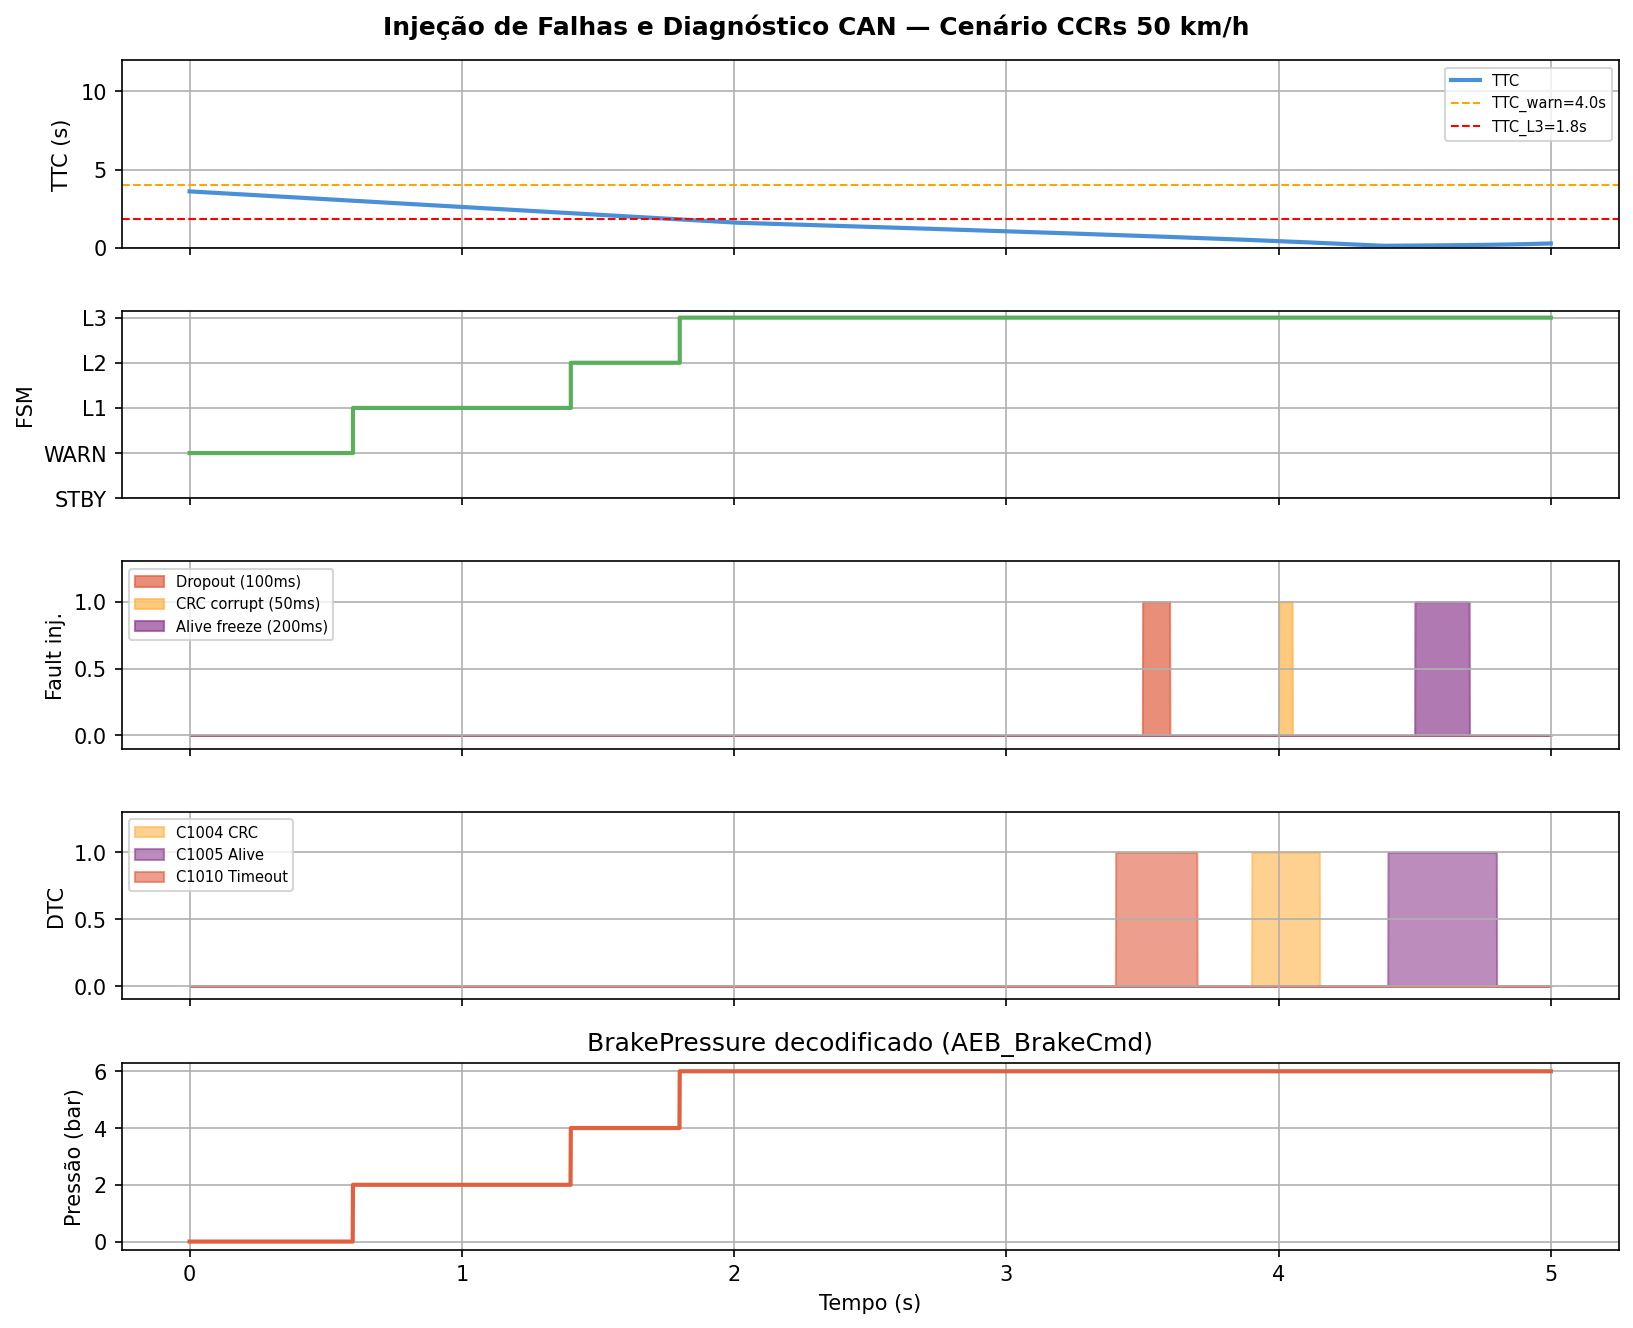
\includegraphics[width=\linewidth]{fig_injecao_falhas.png}
  \caption{Cenário CCRs 50~km/h com injeção de falhas: dropout em
           $t=3{,}5$~s, CRC em $t=4{,}0$~s e alive freeze em
           $t=4{,}5$~s. Os DTCs C1004, C1005 e C1010 são confirmados
           após debounce de 3~ciclos.}
  \label{fig:injecao}
\end{figure}

%% ═══════════════════════════════════════════════════════════════════════════
\section{Diagnóstico CAN}
\label{sec:diagnostico}

O subsistema \texttt{Diagnosticos} implementa a lógica de debounce de
DTCs conforme \texttt{SENSOR\_FAULT\_CYCLES=3} definido em
\texttt{aeb\_config.h}:

\begin{lstlisting}[style=matlab, caption={Debounce de DTC no MATLAB Function DTC\_Logic}]
% Contador por tipo de falha (sobe/desce com histerese)
if crc_err,   cnt_crc   = min(cnt_crc + 1, 5);
else          cnt_crc   = max(cnt_crc - 1, 0); end
% ... idem para alive_err e timeout_err

% DTC confirmado apos 3 ciclos consecutivos
dtc_c1004 = double(cnt_crc   >= 3);  % Erro de CRC
dtc_c1005 = double(cnt_alive >= 3);  % AliveCounter travado
dtc_c1010 = double(cnt_tmo   >= 3);  % Timeout de mensagem
\end{lstlisting}

\begin{center}
\begin{tabular}{clll}
  \toprule
  \textbf{DTC} & \textbf{Condição} & \textbf{Detecção} & \textbf{ISO~14229} \\
  \midrule
  C1004 & CRC recebido $\neq$ CRC calculado & Imediato & ReadDTCInformation 0x19 \\
  C1005 & AliveCounter travado $>$5~ciclos & 3 ciclos & ReadDTCInformation 0x19 \\
  C1010 & Timeout de mensagem $>$10~ms & 3 ciclos & ReadDTCInformation 0x19 \\
  \bottomrule
\end{tabular}
\end{center}

%% ═══════════════════════════════════════════════════════════════════════════
\section{Pipeline do Modelo Simulink}
\label{sec:pipeline}

\begin{figure}[H]
  \centering
  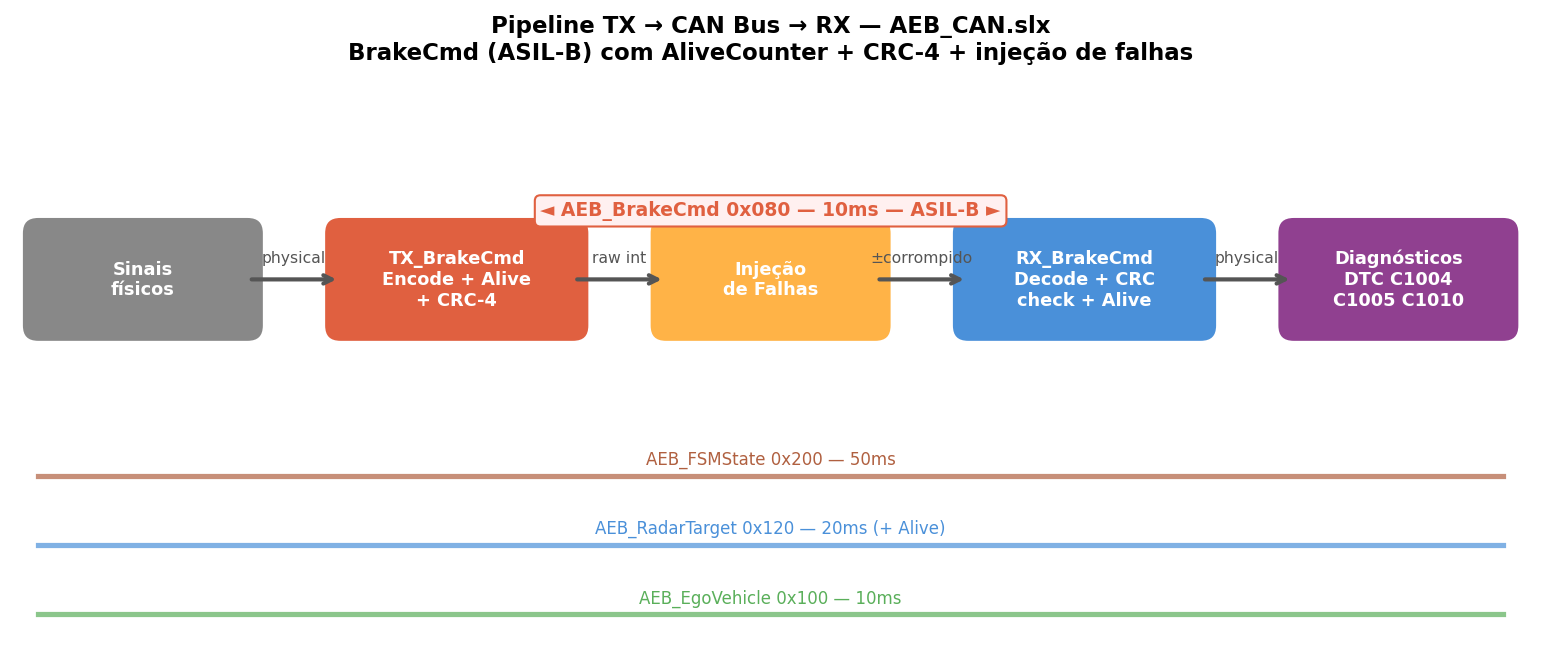
\includegraphics[width=\linewidth]{fig_pipeline.png}
  \caption{Pipeline do modelo \texttt{AEB\_CAN.slx}: o caminho ASIL-B
           (\texttt{AEB\_BrakeCmd}) inclui AliveCounter, CRC-4 e injeção
           de falhas; os demais caminhos usam apenas codificação DBC.}
  \label{fig:pipeline}
\end{figure}

O modelo \texttt{AEB\_CAN.slx} é composto por 12~subsistemas:

\begin{enumerate}
  \item \textbf{TX\_BrakeCmd} --- codificação + AliveCounter + CRC-4
    (10~ms, ASIL-B)
  \item \textbf{TX\_EgoVehicle} --- codificação DBC (10~ms)
  \item \textbf{TX\_RadarTarget} --- codificação + AliveCounter (20~ms)
  \item \textbf{TX\_FSMState} --- codificação DBC (50~ms)
  \item \textbf{TX\_Alert} --- codificação DBC (evento)
  \item \textbf{Injecao\_Falhas} --- dropout, CRC, alive freeze
  \item \textbf{RX\_BrakeCmd} --- decodificação + verificação CRC + alive + timeout
  \item \textbf{RX\_EgoVehicle} --- decodificação DBC
  \item \textbf{RX\_RadarTarget} --- decodificação + verificação alive
  \item \textbf{RX\_FSMState} --- decodificação DBC
  \item \textbf{RX\_Alert} --- decodificação DBC
  \item \textbf{Diagnosticos} --- debounce e confirmação de DTCs
\end{enumerate}

%% ═══════════════════════════════════════════════════════════════════════════
\section{Resultados de Simulação}
\label{sec:resultados}

\subsection{Sinais decodificados --- cenário nominal}

O cenário padrão simula um evento CCRs a 50~km/h (13,89~m/s), com
o AEB ativando frenagem a partir de $t \approx 2$~s quando o TTC
cruza os limiares definidos em \texttt{aeb\_config.h}
($\text{TTC}_{\text{warn}} = 4{,}0$~s,
 $\text{TTC}_{L1} = 3{,}0$~s, $\text{TTC}_{L2} = 2{,}2$~s,
 $\text{TTC}_{L3} = 1{,}8$~s).

\begin{tcolorbox}[notabox]
  A comparação entre os sinais TX e RX decodificados verifica a corretude
  dos fatores e \textit{offsets} do DBC. Para todos os sinais sem injeção
  de falha, $\text{TX} = \text{RX}$ a menos de erros de quantização
  $\leq \text{fator}/2$.
\end{tcolorbox}

\subsection{Parâmetros DBC consolidados}

\begin{figure}[H]
  \centering
  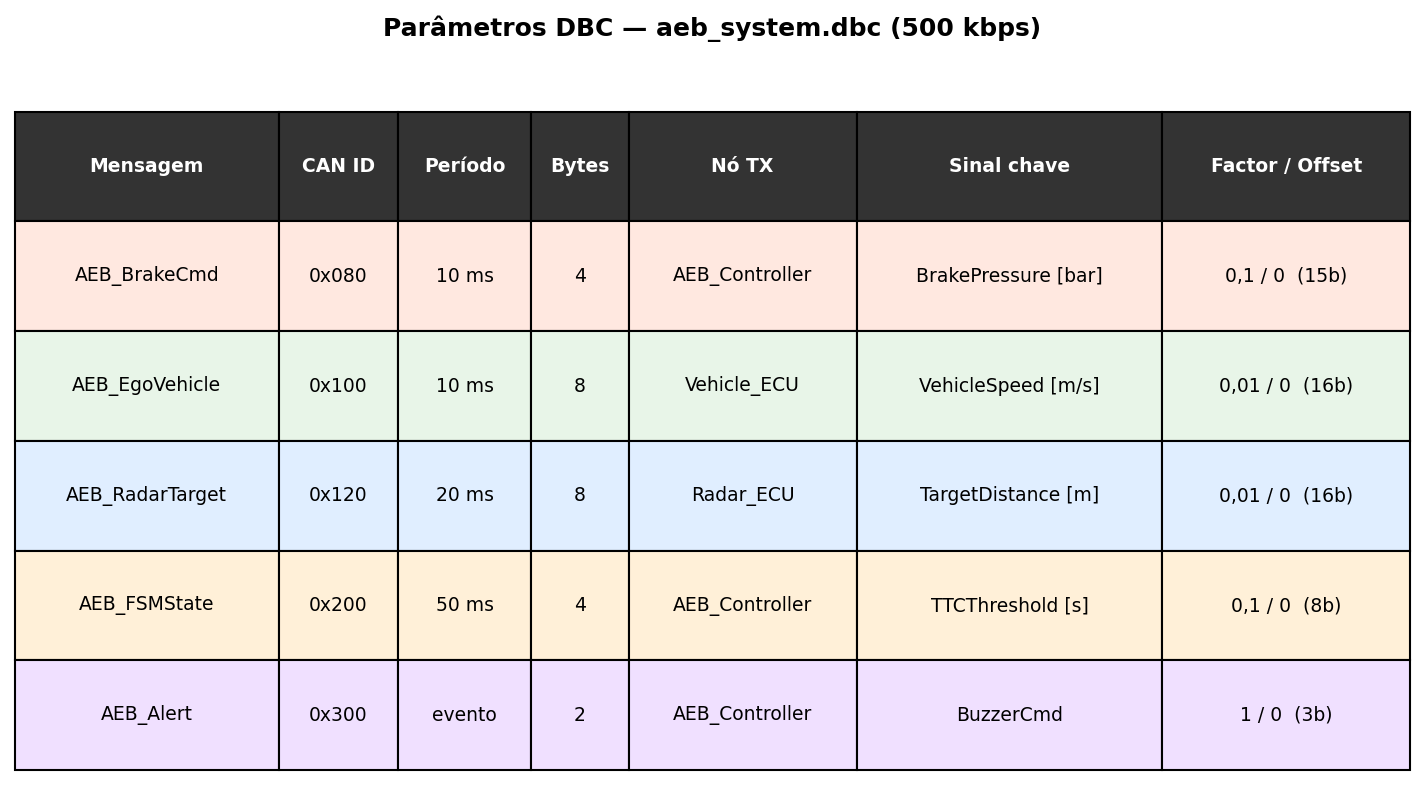
\includegraphics[width=\linewidth]{fig_parametros_dbc.png}
  \caption{Tabela de parâmetros DBC das 5 mensagens CAN do sistema AEB.}
  \label{fig:parametros}
\end{figure}

\subsection{Uso}

\begin{lstlisting}[style=matlab, caption={Uso do modelo AEB\_CAN.slx}]
% 1. Criar o modelo
run('AEB_CAN_build.m')

% 2. Cenario nominal
out = sim('AEB_CAN');
AEB_CAN_plot(out)

% 3. Injetar falha de CRC
AEB_CAN_scenarios('fault_crc')
out = sim('AEB_CAN');
AEB_CAN_plot(out)

% 4. Injetar dropout + alive freeze combinados
AEB_CAN_scenarios('fault_combined')
out = sim('AEB_CAN');
\end{lstlisting}

%% ═══════════════════════════════════════════════════════════════════════════
\section{Sincronização \texttt{v\_target\_cached\_}}
\label{sec:sync}

Um problema sutil de temporização assíncrona ocorre porque
\texttt{AEB\_EgoVehicle} chega a 10~ms e \texttt{AEB\_RadarTarget} a 20~ms.
Se o controlador calculasse
$v_{\text{target}} = v_{\text{ego}} - v_{\text{rel}}$
no ciclo de 10~ms usando o \texttt{relative\_speed} mais recente
(com até 20~ms de atraso) e o \texttt{vehicle\_speed} atual, o resultado
poderia ser inconsistente durante acelerações rápidas:

\begin{tcolorbox}[equacaobox, title={Solução: \texttt{v\_target\_cached\_}}]
\begin{equation}
  v_{\text{target}} = v_{\text{ego}}|_{\text{@radar\_callback}}
                    - v_{\text{rel}}|_{\text{@radar\_callback}}
\end{equation}
$v_{\text{target}}$ é calculado \textbf{dentro do callback do radar},
quando $v_{\text{ego}}$ e $v_{\text{rel}}$ são contemporâneos.
No ciclo de 10~ms, apenas \texttt{v\_target\_cached\_} é passado
para \texttt{aeb\_cycle\_10ms()} --- nunca o \texttt{relative\_speed}
diretamente.
\end{tcolorbox}

%% ═══════════════════════════════════════════════════════════════════════════
\section{Conclusão}
\label{sec:conclusao}

O modelo \texttt{AEB\_CAN.slx} demonstra os princípios fundamentais do
barramento CAN no sistema AEB:

\begin{itemize}[leftmargin=1.5em]
  \item \textbf{Codificação DBC}: conversão física $\leftrightarrow$ raw
    com fator, offset e saturação correta para todos os 5 sinais-chave.
  \item \textbf{AliveCounter}: contador rolante de 4~bits módulo~16 presente
    em \texttt{AEB\_BrakeCmd} e \texttt{AEB\_RadarTarget}; verificação
    instantânea no receptor.
  \item \textbf{CRC-4}: XOR dos campos \texttt{alive}, \texttt{brake\_req}
    e \texttt{brake\_mode}, mascarado em 4~bits --- detecta erros de bit único.
  \item \textbf{Injeção de falhas}: três tipos controláveis (dropout, CRC
    corrupto, alive freeze) com janelas de tempo configuráveis.
  \item \textbf{Diagnóstico}: debounce de 3~ciclos para confirmação dos
    DTCs C1004, C1005 e C1010, compatível com ISO~14229.
\end{itemize}

\begin{tcolorbox}[notabox]
  \textbf{Vehicle Network Toolbox}: com o toolbox disponível, os blocos
  nativos \texttt{CAN Pack} / \texttt{CAN Unpack} podem importar
  \texttt{aeb\_system.dbc} diretamente, substituindo os blocos
  MATLAB Function de codificação. A arquitetura de subsistemas e a lógica
  de AliveCounter/CRC permanecem idênticas.
\end{tcolorbox}

\vspace{1cm}
\noindent\rule{\linewidth}{0.4pt}\\[0.2cm]
{\small\color{cinza}
Residência Tecnológica Stellantis/UFPE 2026 ---
Gerado com MATLAB R2025b + Simulink + tectonic v0.15.0}

\end{document}
